\subsection{Fisher method}
\begin{figure}
	\centering		
	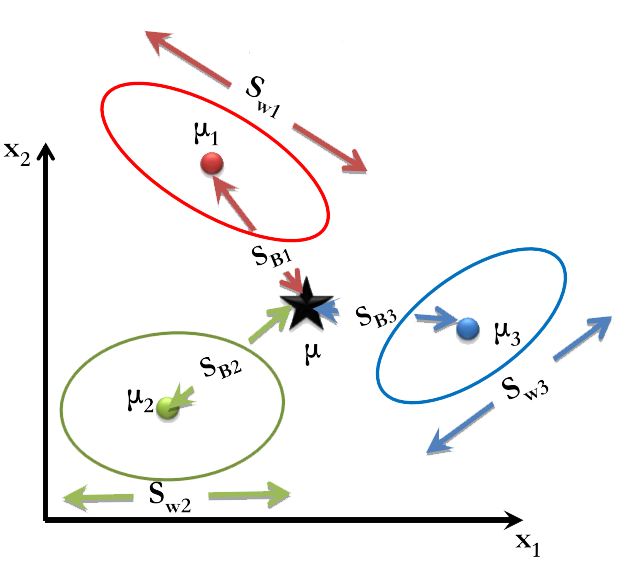
\includegraphics[width = 0.4\textwidth]{rsrc/LDA_basic.png}
	\caption{Az LDA algoritmus által megvizsgált szórások. The source of the image: \cite{LDA}}
	\label{fig:LDA abrazolas}
\end{figure}

Ha $ m $ dimenziós vektorokat szeretnék leképezni egy $ C $-dimenziós térbe akkor azt a következő módon tehetem meg.
\begin{equation}
y = w^Tx \textrm{, where } 
\end{equation}
\begin{equation}
x = \left(
\begin{array}{ccc}
x_1\\
\vdots\\
x_m
\end{array} \right)
w=\left(
\begin{array}{ccc}
w_{1,1} \dots w_{1,C}\\
\vdots \ddots \vdots\\
w_{m,1} \dots w_{m,C}
\end{array}
\right)
y = \left(
\begin{array}{ccc}
y_1\\
\vdots\\
y_C
\end{array}\right)
\label{equ:Alap_egyenlet}
\end{equation}